%%%%%%%%%%%%%%%%%%%%%%%%%%%%%%%%%%%%%%%%%%%%%%%%%%%%%%%%%%%%%%%%%%%%%%%%%
%									%
% %CS_383_Assignment4_LaTeX_Design_Specification_Components_Adrian	%
% LaTeX Template							%
% Version 1.2 (3/7/17)							%
%									%
%									%
% author: Adrian Beehner						%
%									%
%									%
% description: LaTeX document that contains part of the			%
%  component overview of the design specificaiton			%
%									%
%%%%%%%%%%%%%%%%%%%%%%%%%%%%%%%%%%%%%%%%%%%%%%%%%%%%%%%%%%%%%%%%%%%%%%%%%


% Set Up Document
\documentclass[12pt]{article}
\usepackage{titlesec} 
\usepackage{hyperref}
\usepackage{graphicx}
\usepackage{float}
\usepackage{parskip} % Adds spacing between paragraphs
\setlength{\parindent}{15pt} % Indent paragraphs (automatically)

% This probably doesn't corelate to everyone else's so its fine to get rid of it (I like the margins futher out personally)
\usepackage[margin=1in]{geometry}

% Make so Picture/floats go at top of page (So it doesn't waste any whitespace on document)
\makeatletter
\setlength{\@fptop}{0pt}
\makeatother


\begin{document}
	
	% Set up Manual Indenting (isn't essential - I once again used it for my own prefernces)
	\setlength{\parindent}{15pt}
	\newcommand{\forceindent}{\leavevmode{\parindent=2em\indent}}
	
	%----------------------------------------------------------------------------------------
	%	SECTIONS
	%----------------------------------------------------------------------------------------

	%----------------------------------------------------------------------------------------
	%	SECTION 1 Content
	%----------------------------------------------------------------------------------------
	\section{Test}
	\forceindent 	
			
	% Create new Page (NEED TO USE clearpage because of the pictures that will affect it! - /newpage wont work on the pictures)
	\clearpage
	

	%----------------------------------------------------------------------------------------
	%	SECTION 2 Content
	%----------------------------------------------------------------------------------------
	\section{Program Overview/Scope}
	\forceindent The system software we are designing is being developed with scalability in mind. The goal is to create a Framework that can be updated and scaled easily, and to some degree, efficiently. Changes in the following development phases in the coming weeks will require adding the basic framework (the editor itself), then adding different types of functionality such as a different set of editors, such as single vs. multiple nodes editors (nodes represent the individual goofy glasses on the marching band members). There will a graphical user interface (GUI) that allows the manipulation of the colors of each node, multiple nodes, or a manipulation grid large enough to allow movement of the entire set of nodes. The manipulation grid, as well as the number of nodes should be variable (yet reside at a default value unless the user specifies). We will assume that no nodes in the grids are allowed to change places, all nodes must reside in their original location (in regards to their relative position to other nodes). Another assumption is that the glasses themselves are already setup with a \textit{n} nodes channel receiver (for each node, \textit{n} = 150 glasses for the marching band), as there are a total of \textit{n} glasses, thus implying there is at least a 3\textit{n}-byte receiver (\textit{n} channels, each can send a 3 byte message-for RGB). The program will be able to run on any Operating System with Java installed, with no changes in the functionality of the program, each OS will utilize its own specific file system properties when the system software must handle saving the projects of the system software.
	
		% Subsections
		%----------------------------------------------------------------------------------------
		%	COMPONENT OVERVIEW
		%----------------------------------------------------------------------------------------
		\subsection {Component Overview}
		\forceindent There are seven main components in the system software, which include the Configuration Editor, the Single Node editor, the Mulit-Node Editor, Grid Editor, Character Editor, Animation Creator, and File Generator. The Configuration Menu Bar which will provide a simple interface for setting up and/or configuring the grid and glasses, as well as saving a project. The Single Node Editor will provide the user with an interface to edit single Nodes individually. The Multi-Node Editor will provide the user with an interface to edit multiple (possibly all) Nodes individually. The Grid Editor will provide the user with an interface to edit a scalable grid that contains space larger than the current specified/defualt amount of nodes. The Character Edit will provide the user with an interace for the creaton, editing, and saving of any special grid formations, with default numbers and letters existing within the editor. The Animator Creator will allow the user to create animations with the characters from the Character Animator, allowing the user to create animations via corresponding grid(s). The File Generator is an simple interface that allows the text representation of the animation created in a program to be a saved to a \textit{tan} file format. way the user will utilize the 4 basic components (Configuration Editor, the Single Node editor, the Mulit-Node Editor, Grid Editor) is shown in Figure 1:
		
		\begin{figure}[ht!]
			\centering
			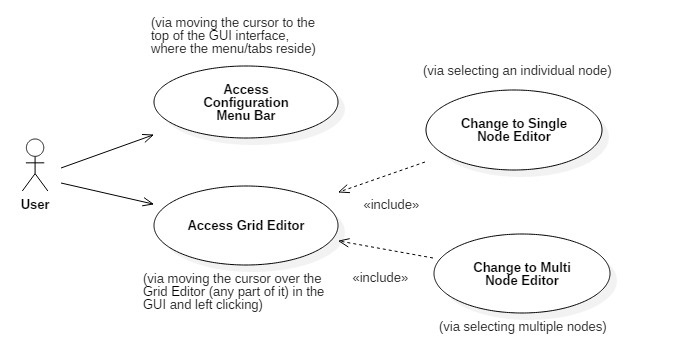
\includegraphics[width=170mm]{ComponetOverview.JPG}
			\caption{Use Case Diagram of "Basic" Component Overview \label{overflow}}
		\end{figure}
		
			% Subsubsections
			%----------------------------------------------------------------------------------------
			%	CONFIGURATION
			%----------------------------------------------------------------------------------------
			\subsubsection {Configuration Menu Bar}
			\forceindent The configuration menu bar will provide a simple interface via a horizontal menu bar at the top of the GUI that provides the user with various options on how they wish to configure the number of glasses, grid size, and checking/changing the pairing of the glasses. The number of glasses option will provide a simple diaglog box to enter the number of glasses/nodes the user wishes to use (and adjust the grid accordingly). The grid size option will also provide a diaglog box that allows the user to select a grid dimension (the grid dimensions will only be allowed if all the n nodes can fit within that space, otherwise a error will be thrown). There will able be a file option/tab that allows the user to open, create a new project, save, or save as for a project. %Finally, the checking/configuring glasses options will provide a simple display that shows how many glasses are connected, as well as having a drop down box option to pairing up glasses, which will then provide a dialog box to pair/edit glasses (via the receivers rotary switch on the glasses).
		    The only inputs are from putting the cursor over the tabs and clicking on them to access their dialog boxes/displays as mentioned above. This component controls how the grid editor components dimensions are made up, and does have a component that it relies on to function properly. There should be some CPU-memory intensiveness for the tasks under this component, such as registering the number of Nodes/Glasses, changing the grid dimensions, and pairing glasses can all become intensive if the numbers are large enough, and general overhead due to GUI can occur. The general use-case of this component is shown in Figure 2.
			
			\begin{figure}[ht!]
				\centering
				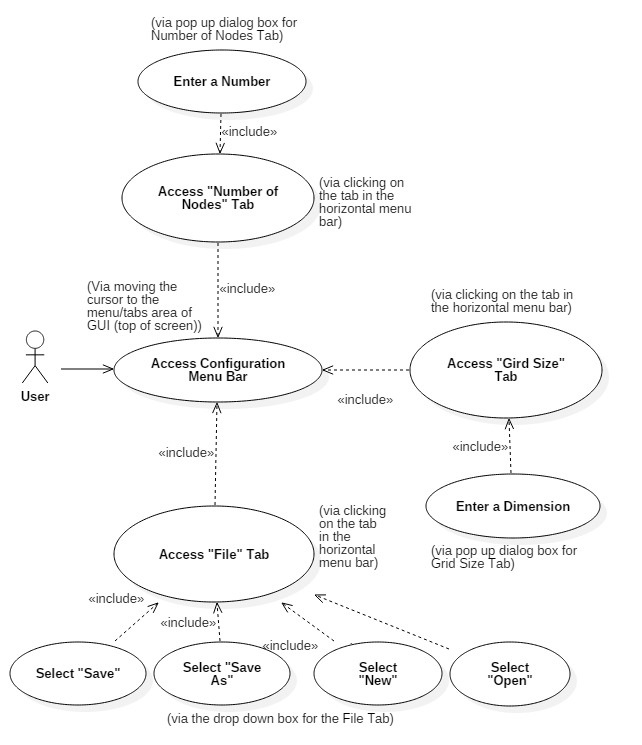
\includegraphics[width=170mm]{Configuration_Editor.JPG}
				\caption{Use Case Diagram of the Configuration Menu Bar \label{overflow}}
			\end{figure}
			
			%----------------------------------------------------------------------------------------
			%	SINGLE NODE EDITOR
			%----------------------------------------------------------------------------------------
			\subsubsection {Single Node Editor}
			\forceindent The Single Node Editor in the system software will allow the user to edit any individual node via a user interface. This means the user can hand pick various nodes and set specific colors to them. Thus the component allows the user to edit any individual node on the grid, choose a color via a color dialog box, and see the feedback via the grid Editor. The only inputs are from clicking on the individual node and then click on a color via the dialog box, and the output is displaying the color dialog box, and displaying the node with the chosen color. This component relies on the Grid Editor (who displays the nodes) for providing an interface. Constraints of this program are that it cannot be changed from this mode when editing a node is in process, and thus no other actions (in the system software) may be performed while editing a node (or the component will actually exit editing the node without applying any changes). There should not be any CPU-memory-intensiveness for task under this component, overhead may occur due to the GUI however. The general use-case of this component can be seen below in Figure 3.
			
			\begin{figure}[ht!]
				\centering
				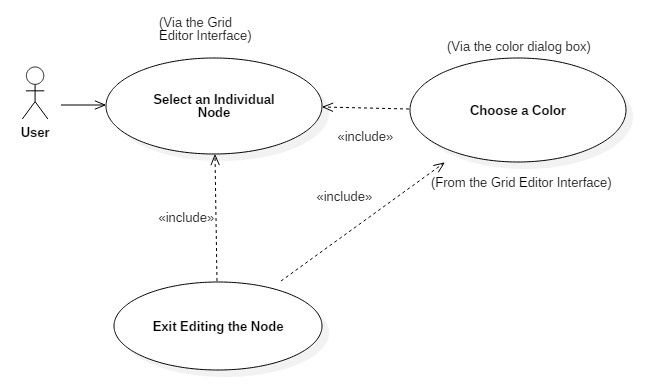
\includegraphics[width=150mm]{SingleNodeEditorDiagram.JPG}
				\caption{Use Case Diagram of Single Node Editor \label{overflow}}
			\end{figure}
		
			%----------------------------------------------------------------------------------------
			%	MULTI NODE EDITOR
			%----------------------------------------------------------------------------------------
			\subsubsection {Multi Node Editor}
			\forceindent 
			
			%----------------------------------------------------------------------------------------
			%	GRID EDITOR
			%----------------------------------------------------------------------------------------
			\subsubsection {Grid Editor}
			\forceindent 
			
		
		%----------------------------------------------------------------------------------------
		%	COMPONENT RELATIONSHIP
		%----------------------------------------------------------------------------------------
		\subsection {Component Relationship}
		\forceindent 

		
	\end{document}
